\subsection{Otras observaciones de interés}

\subsubsection{Análisis de varianza del método propuesto}

Con el fin de analizar la estabilidad del método y poner en perspectiva sus resultados en comparación con los algoritmos del estado del arte, se realiza un \textit{análisis de varianza} (ANOVA del inglés \textbf{An}alysis \textbf{o}f \textbf{Va}riance) y se aplica el \textit{método de Tukey} a continuación.

\bigskip El análisis de varianza prueba la significancia estadística de la diferencia de medias (o tendencia central) entre los diferentes métodos en análisis. Si la diferencia entre las medias es estadísticamente significativa, significa que la diferencia esperada es probable que reaparezca si los experimentos son realizados nuevamente \citep{tabachnick2007experimental}. El término \textit{estadísticamente significativo} indica que rechazar la hipótesis nula no significa que el hallazgo sea importante, sino que la diferencia media es lo suficientemente grande como para que la muestra vuelva a aparecer si los experimentos son realizados nuevamente. En el caso de estudio, considerando la media de error como variable en análisis, la hipótesis nula sugiere que el método EQuAL es apto, eficiente y eficaz para ser utilizado en un sistema de recomendación, en comparación con métodos aptos y reconocidos por la comunidad. Para clarificar, la intención de este trabajo es aceptar la hipótesis nula o, aun mejor, rechazar la hipótesis nula con una medida de rendimiento que demuestre que el método EQuAL es estadísticamente mejor. En este apartado se usa el análisis de varianza como una herramienta para tal fin. Si los resultados son los esperados, podemos llegar a la conclusión que el método EQuAL puede ser utilizado como medio para generar matrices de similaridad aptas para un RS eficiente y eficaz, mediante pruebas estadísticamente significativas. Se realizó un estudio ANOVA\footnote{El código completo del análisis de varianza se encuentra en este repositorio GitHub \url{https://github.com/fedetesone/anova_equal}.} con los datos\footnote{Conjunto de datos fuente para el análisis de varianzas: \url{https://github.com/fedetesone/anova_equal/blob/main/resultados.csv}.} utilizados para generar las tablas resumen del apartado “\ref{ss:analisismetodoestado} Análisis del método propuesto y algoritmos del estado del arte”.

\bigskip Los algoritmos del estado del arte y método EQuAL basado en el ensamble de los mismos, generaron conjuntos de datos que son utilizados como entrada para el análisis de varianza. Los conjuntos de datos de los métodos del estado del arte se toman como \textit{grupos base}, y el conjunto de datos del método EQuAL es el grupo variable (o también \textit{factor variable}). Se plantean las siguientes hipótesis:
\begin{itemize}
	\item \textbf{\(H_0\)}: La media de los valores de error de los métodos en estudio para un tamaño de muestra determinado, es estadísticamente igual.
	\item \textbf{\(H_1\)}: La media de los valores de error de los métodos en estudio para un tamaño de muestra determinado, es significativamente diferente.
\end{itemize}

\bigskip Se va a aplicar la técnica \textit{ANOVA de un factor}, que relaciona dos variables: el método aplicado a la muestra aleatoria (independiente) y el valor de error obtenido (dependiente). La variable dependiente es el llamado \textit{factor}. Sin embargo, el análisis de medias de error a continuación se realizará comparando el método EQuAL contra los métodos del estado del arte (uno a uno), para un tamaño de muestra determinado. Para tal fin, se utiliza el método de Tukey para crear intervalos de confianza para todas las diferencias de medias, en parejas. El motivo por el cual es realizado de esta forma es porque el método ANOVA indica que al menos un grupo (cualquiera de ellos) difiere de los demás. Por lo anterior, para un análisis más específico, es necesario el énfasis especial es el método propuesto realizando comparaciones específicas mediante pares \citep{abdi2010tukey}. Por ejemplo, si el método ANOVA arroja que hay diferencias significativas entre las medias en análisis, el método de Tukey puede aplicarse para saber específicamente donde radican las mismas. Filtrando las comparaciones uno a uno en las cuales se encuentra el método EQuAL, es posible saber cómo se comporta. Si las medias de error son iguales en términos estadísticos, significa que el método EQuAL es, al menos, apto para la generación de medidas de similaridad a partir del conjunto de datos en estudio, y su aplicación en RS.

\bigskip A continuación, se muestran los métodos ANOVA y Tukey aplicados en R para cada uno de los tamaños de muestra tenidos en cuenta en los experimentos, utilizando un nivel de confianza de \(95\%\) (\(\alpha = 0.05\)).

\paragraph{Tamaño de muestra de 100 pares de preguntas}

\begin{rc}
                 Df  Sum Sq  Mean Sq F value Pr(>F)
as.factor(metodo)  5 0.00938 0.001875   0.731  0.603
Residuals         54 0.13851 0.002565
\end{rc}

\begin{rc}
                 diff        lwr       upr     p adj
ensemble-bow     0.008 -0.0589175 0.0749175 0.9992360
ft-ensemble      0.030 -0.0369175 0.0969175 0.7702455
gtfidf-ensemble  0.007 -0.0599175 0.0739175 0.9996012
sem-ensemble    -0.003 -0.0699175 0.0639175 0.9999940
w2v-ensemble     0.013 -0.0539175 0.0799175 0.9923331
\end{rc}

\begin{figure}
	\centering
	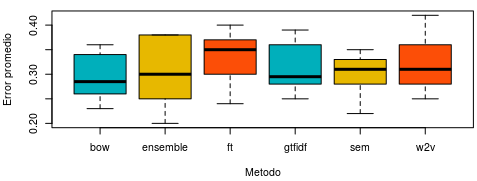
\includegraphics[width=0.7\linewidth]{10_resultados/imagenes/anova_100}
	\caption{Gráfico de caja y bigote para las medias de error de los métodos en estudio para tamaño de muestra de 100 pares de preguntas.}
	\label{fig:anova100}
\end{figure}

\begin{itemize}
	\item \(P_r(F) = 0.603 > \alpha, \alpha = 0.05\) indica que no hay una diferencia significativa en el conjunto total. No se rechaza la hipótesis nula.
	\item El método EQuAL posee una media de error estadísticamente igual a todos los métodos. En todos los casos, los intervalos de confianza incluyen al valor 0 y \(p-adj > \alpha\)
	\item El método EQuAL posee el menor valor de error para una ejecución en particular, representado por el bigote inferior.
\end{itemize}

\paragraph{Tamaño de muestra de 500 pares de preguntas}

\begin{rc}
                 Df   Sum Sq   Mean Sq F value Pr(>F)
as.factor(metodo)  5 0.001938 0.0003876   1.983 0.0959 .
Residuals         54 0.010554 0.0001954
\end{rc}

\begin{rc}
                  diff          lwr         upr     p adj
ensemble-bow     0.0018 -0.016671384 0.020271384 0.9997181
ft-ensemble      0.0142 -0.004271384 0.032671384 0.2237050
gtfidf-ensemble  0.0078 -0.010671384 0.026271384 0.8113536
sem-ensemble     0.0036 -0.014871384 0.022071384 0.9922183
w2v-ensemble     0.0106 -0.007871384 0.029071384 0.5407045
\end{rc}

\begin{figure}
	\centering
	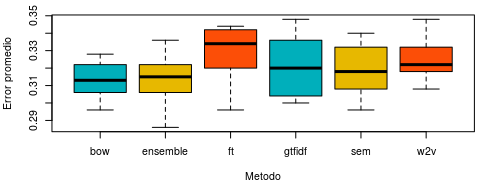
\includegraphics[width=0.7\linewidth]{10_resultados/imagenes/anova_500}
	\caption{Gráfico de caja y bigote para las medias de error de los métodos en estudio para tamaño de muestra de 500 pares de preguntas.}
	\label{fig:anova500}
\end{figure}

\begin{itemize}
	\item \(P_r(F) = 0.0959 < \alpha, \alpha = 0.05\) indica que hay una diferencia significativa en el conjunto total. Se rechaza la hipótesis nula.
	\item El método EQuAL posee una media de error estadísticamente igual a todos los métodos. En todos los casos, los intervalos de confianza incluyen al valor 0 y \(p-adj > \alpha\)
	\item El método EQuAL posee el menor valor de error para una ejecución en particular, representado por el bigote inferior.
\end{itemize}

\paragraph{Tamaño de muestra de 1000 pares de preguntas}

\begin{rc}
                 Df   Sum Sq   Mean Sq F value Pr(>F)
as.factor(metodo)  5 0.002585 0.0005170   1.924  0.105
Residuals         54 0.014514 0.0002688
\end{rc}

\begin{rc}
                  diff          lwr         upr     p adj
ensemble-bow     0.0175 -0.004161633 0.039161633 0.1791584
ft-ensemble     -0.0049 -0.026561633 0.016761633 0.9846755
gtfidf-ensemble -0.0072 -0.028861633 0.014461633 0.9217004
sem-ensemble    -0.0162 -0.037861633 0.005461633 0.2504112
w2v-ensemble    -0.0155 -0.037161633 0.006161633 0.2956972
\end{rc}

\begin{figure}
	\centering
	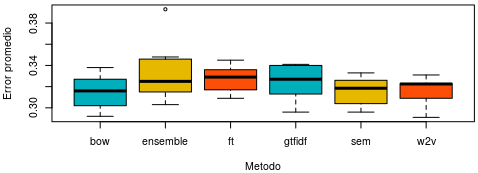
\includegraphics[width=0.7\linewidth]{10_resultados/imagenes/anova_1000}
	\caption{Gráfico de caja y bigote para las medias de error de los métodos en estudio para tamaño de muestra de 1000 pares de preguntas.}
	\label{fig:anova1000}
\end{figure}

\begin{itemize}
	\item \(Pr_(F) = 0.105 > \alpha, \alpha = 0.05\) indica que no hay una diferencia significativa en el conjunto total. No se rechaza la hipótesis nula.
	\item El método EQuAL posee una media de error estadísticamente igual a todos los métodos. En todos los casos, los intervalos de confianza incluyen al valor 0 y \(p-adj > \alpha\)
\end{itemize}

\paragraph{Tamaño de muestra de 1500 pares de preguntas}

\begin{rc}
                 Df   Sum Sq   Mean Sq F value Pr(>F)
as.factor(metodo)  5 0.001514 0.0003027   2.936 0.0214 *
Residuals         49 0.005053 0.0001031
\end{rc}

\begin{rc}
                        diff           lwr         upr     p adj
ensemble-bow     0.0090666667 -7.427521e-03 0.025560854 0.5832109
ft-ensemble      0.0027333333 -1.376085e-02 0.019227521 0.9962642
gtfidf-ensemble  0.0028666667 -1.362752e-02 0.019360854 0.9953275
sem-ensemble     0.0044666667 -1.202752e-02 0.020960854 0.9656207
w2v-ensemble    -0.0062000000 -2.269419e-02 0.010294187 0.8729702
\end{rc}

\begin{figure}
	\centering
	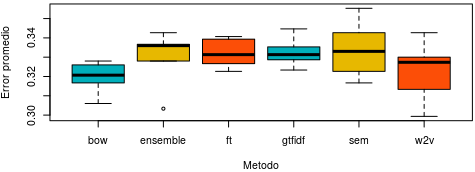
\includegraphics[width=0.7\linewidth]{10_resultados/imagenes/anova_1500}
	\caption{Gráfico de caja y bigote para las medias de error de los métodos en estudio para tamaño de muestra de 1500 pares de preguntas.}
	\label{fig:anova1500}
\end{figure}

\begin{itemize}
	\item \(P_r(F)= 0.0214 < \alpha, \alpha = 0.05\) indica que hay una diferencia significativa en el conjunto total. Se rechaza la hipótesis nula.
	\item El método EQuAL posee una media de error estadísticamente igual a todos los métodos. En todos los casos, los intervalos de confianza incluyen al valor 0 y \(p-adj > \alpha\)
	\item En este caso, es de vital importancia la comparación en parejas, teniendo como foco el método EQuAL; ya que, si bien la hipótesis nula fue rechazada, la comparación individual del mismo con los algoritmos del estado del arte, no muestra una diferencia significativa.
\end{itemize}

\paragraph{Tamaño de muestra de 2000 pares de preguntas}

\begin{rc}
                 Df   Sum Sq   Mean Sq F value   Pr(>F)
as.factor(metodo)  5 0.002348 0.0004697   6.144 0.000171 ***
Residuals         49 0.003746 0.0000765
\end{rc}

\begin{rc}
                  diff       lwr       upr      p adj
ensemble-bow     0.01585  0.001648 0.0300516 0.020523
ft-ensemble      0.00385 -0.010351 0.0180516 0.965462
gtfidf-ensemble -0.00035 -0.014551 0.0138516 0.999999
sem-ensemble    -0.00570 -0.019901 0.0085016 0.839375
w2v-ensemble    -0.00725 -0.021451 0.0069516 0.657185
\end{rc}

\begin{figure}
	\centering
	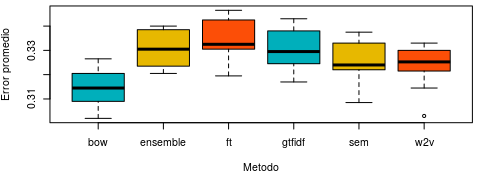
\includegraphics[width=0.7\linewidth]{10_resultados/imagenes/anova_2000}
	\caption{Gráfico de caja y bigote para las medias de error de los métodos en estudio para tamaño de muestra de 2000 pares de preguntas.}
	\label{fig:anova2000}
\end{figure}

\begin{itemize}
	\item \(P_r(F)= 0.000117 < \alpha, \alpha = 0.05\) indica que hay una diferencia significativa en el conjunto total. Se rechaza la hipótesis nula.
	\item En este caso, el rechazo de la hipótesis nula es causado por el método Bow, que tuvo muy buenos indicadores en este tamaño de muestra. Si el mismo no fuese tenido en cuenta para este tamaño de muestra, el indicador \(P_r(F)\) hubiese sido  \(P_r(F)= 0.056 > \alpha\) que indicaría que no hay diferencia entre los métodos analizados. Por lo anterior, el método EQuAL tiene una diferencia significativa solo con el método bow, siendo estadísticamente igual a los restantes.
\end{itemize}

\bigskip En general, el método EQuAL tiene un comportamiento aceptable en cuanto a medias de error a lo largo de todos los tamaños de muestra. Esto significa que las medias de error del mismo son significativamente comparables con los métodos del estado del arte, los cuales son utilizados por la comunidad en el cálculo de similaridad y análisis de texto, e inclusive superador en algunos casos.

\subsubsection{Desempeño con tamaños de muestra pequeños}
En el análisis de varianza de las medias de error realizado anteriormente, se puede observar que el método EQuAL se comporta muy bien en los tamaños de muestra de 100 y 500 pares de preguntas: el método propuesto fue estadísticamente igual o superior a los métodos del estado del arte. Sin embargo, para tamaños de muestra más grandes, fue superado en algunas oportunidades.

\bigskip Esto demuestra que el agregado de variabilidad de datos puede ser influyente en el cálculo de similaridad. Los métodos del estado del arte cada una de las preguntas de cada para entre sí, mientras que el método EQuAL realiza una comparación “todas contra todas” con el objetivo de realizar un método de clustering a continuación. Para clarificar, se puede concluir que los gráficos y estadísticas obtenidos muestran que métodos basados en ensamble de clustering, y en particular el método EQuAL,  proponen una medida de similaridad adimensional que puede mejorar ciertas medidas de rendimiento en comparativa con otros algoritmos. Citando a \cite{fred2005combining} esta mejora se hace aún más evidente en tamaños de muestras chicos o conjuntos de datos complejos.

\subsubsection{Dependencia de un método de ensamble con sus algoritmos subyacentes}
Si bien es una medida adimensional y propone mejorar las medidas de rendimiento en ciertos aspectos, los métodos de ensamble de clustering son dependientes de sus algoritmos subyacentes y, por lo tanto, las medidas de desempeño son similares en cuanto a, por ejemplo, el valor de error obtenido. Los análisis de varianza realizados ponen en evidencia la dependencia del método equal con los algoritmos ensamblados. La media de error es la misma (estadísticamente hablando) en la mayoría de los casos, lo cual indica que los valores arrojados por el método de ensamble son directamente proporcionales a las medias subyacentes, dando la posibilidad de mejorar los indicadores de rendimiento cuando se utilicen algoritmos de similaridad de texto que tengan mejor comportamiento.

\subsubsection{Influencia del conjunto de datos Quora}
En las secciones anteriores se demostró que el método EQuAL es apto para la utilización en un sistema de recomendación. No obstante, no posee ventajas claras sobre los métodos del estado del arte en algunas medidas de rendimiento en particular.

\bigskip El conjunto de datos Quora y la naturaleza del mismo, no permite realizar un diagrama de dispersión que posibilite ver la forma de los clusters generados. Dicho esto, y sabiendo que la técnica de Ensamble de Clustering es particularmente efectiva en la detección de clusters con formas no convencionales, no es posible identificar fácilmente cuál es la forma de los clusters en cuestión, y verificar si el método EQuAL se adapta perfectamente al conjunto de datos.

\bigskip Por otro lado, el conjunto de datos compara preguntas una a una, que generalmente tienen una o más palabras en común. Esto provoca que los métodos como TF o TFIDF que cuantifican la cantidad de palabras en común, se comporten relativamente bien o arrojen, al menos, un  resultado distinto de cero que supera a los métodos “más inteligentes”. Lo contrario ocurriría, si la comparación de texto fuese entre frases cortas que utilicen sinónimos o palabras completamente distintas, donde los algoritmos basados en taxonomías y técnicas de ML tendrían clara ventaja.

\bigskip El método EQuAL, no es únicamente efectivo para algoritmos subyacentes basados en análisis de texto, sino que también es posible utilizarlo para cualquier conjunto de datos y técnica que generen matrices de distancia como salida. Tal es así, que podría funcionar de manera excepcional con conjuntos de datos que puedan ser graficados y tengan clusters identificables visualmente, con formas que sean convenientes para métodos basados en Ensamble de Clustering.
